\documentclass[usenames,dvipsnames]{beamer}


\usetheme{Madrid}
\usecolortheme{dolphin}
\setbeamercolor{title}{fg=NavyBlue}
\setbeamercolor{frametitle}{fg=NavyBlue}
\setbeamercolor{section in toc}{fg=NavyBlue}

%\AtBeginEnvironment{theorem}{%
%	\setbeamercolor{block title}{fg=white,bg=NavyBlue}
%}

\usepackage{amsthm}
\usepackage{graphicx}
\usepackage[utf8x]{inputenc}
\usepackage{mathtools}
\mathtoolsset{showonlyrefs}
\usepackage{appendixnumberbeamer}
\usepackage{enumitem}
\usepackage{centernot}
\usepackage{tikz}
\usepackage[lined]{algorithm2e}
\usepackage{caption}
\usetikzlibrary{positioning}
\setitemize{label=-, leftmargin=*}
\usepackage{booktabs}

\DeclarePairedDelimiter{\abs}{\lvert}{\rvert}
\DeclarePairedDelimiter{\norm}{\|}{\|}
\renewcommand{\Pr}{\mathbb{P}}
\newcommand{\R}{\mathbb{R}}
\newcommand{\Var}{\operatorname{Var}}
\newcommand{\E}{\operatorname{\mathbb{E}}}
\newcommand{\iid}{\ensuremath{\stackrel{\text{iid}}{\sim}}}
\renewcommand{\phi}{\varphi}
\renewcommand{\theta}{\vartheta}
\newcommand{\epl}{\varepsilon}

% Theorem blocks
\newenvironment<>{greenblock}[1][]{%
\setbeamercolor{block title}{fg=white,bg=ForestGreen}%
\begin{block}#2{#1}}{\end{block}}
\newenvironment<>{redblock}[1][]{%
\setbeamercolor{block title}{fg=white,bg=red!75!black}%
\begin{block}#2{#1}}{\end{block}}

% Add numbers and take out navigation symbols
\setbeamertemplate{footline}[frame number]
\beamertemplatenavigationsymbolsempty

% Text starts always from the top of the frame
\newenvironment{frameT}{\begin{frame}[t]}{\end{frame}}

\title{Probabilistic methods for uncertainty quantification of the error in	numerical solvers of differential equations}
\author{Assyr Abdulle, \underline{Giacomo Garegnani}}
\date{Candidacy Exam, 20 March 2018}
\institute[EPFL]{
\includegraphics[width=3cm]{Logo}}

\AtBeginSection[]
{
	\begin{frame}<beamer>
	\frametitle{Outline}
		\tableofcontents[currentsection]
	\end{frame}
}


\begin{document}
	
\thispagestyle{empty}
\frame{\titlepage}

\begin{frame}
	\frametitle{Outline}
	\tableofcontents
\end{frame}


\section{Motivation}

\begin{frameT}
	\frametitle{Probabilistic methods -- why?}
	
	Consider Lorenz equation (atmospheric convection)
	\begin{align*}\label{eq:Lorenz}
		x' &= \sigma(y - x),  &&x(0) = -10,\\
		y' &= x(\rho - z) - y,  &&y(0) = -1,\\
		z' &= xy - \beta z,  &&z(0) = 40.
	\end{align*}
	For $\rho=28$, $\sigma=10$, $\beta=8/3$ {\color{BrickRed} chaotic behaviour}.
	
	\vspace{0.2cm}
	$\implies$ Numerical integration gives {\color{BrickRed} unreliable solutions}.
	
	\vspace{1cm}
	\only<2>{
	\begin{greenblock}[Goal]
		Establish a probability measure over the numerical solution given by classical methods.
	\end{greenblock}
	}

\end{frameT}

\begin{frameT}
	\frametitle{Probabilistic methods -- why?}
	
	\begin{figure}
		\begin{center}
			\hspace{-0.15cm}\includegraphics[width=\linewidth]{Lorenz}
		\end{center}
	\end{figure}	

	Time evolution of the first component of Lorenz equation \\
	\makebox[2cm]{\textbf{Black line}} $\to$ deterministic solution \\
	\makebox[2cm]{\color{gray} Gray lines} $\to$ probabilistic solutions. 
	
	\only<2>{\vspace{0.5cm}
	{\color{BrickRed}Chaotic behaviour appears frequently in nonlinear differential equations.}
	}
\end{frameT}

%%%%%%%%%%%%%%%%%%%%%%%
% Probabilistic methods for ODEs

\section{Probabilistic methods for ODEs}

\begin{frameT}
	\frametitle{Notation}
	Autonomous dynamical system, function $f\colon\R^d\to\R^d$ and the ODE
	\begin{equation}
	y' = f(y), \quad y(0) = y_0.
	\end{equation}
	Flow of the equation $\phi_t\colon\R^d\to\R^d$ such that
	\begin{equation}
	y(t) = {\color{ForestGreen}\phi_t(y_0)}.
	\end{equation}
	One-step method: numerical flow $\Psi_h$ such that
	\begin{equation}\label{eq:NumericalFlow}
	y_{n+1} = {\color{NavyBlue}\Psi_h(y_n)}.
	\end{equation}
	Runge-Kutta methods: flow implicitly defined by
	\begin{align}
		K_i &= y_n + h \sum_{j=1}^{s} a_{ij} f(K_j), \\
		{\color{NavyBlue}\Psi_h(y_n)} &= y_n + h \sum_{i=1}^{s} b_i f(K_i).
	\end{align}
\end{frameT}

\begin{frame}
	\frametitle{Probabilistic methods for ODEs}
	
	\only<1>{
		{\color{ForestGreen} Filtering} methods for ODEs: fix a prior on $y(t)$ (Gaussian process), update with evaluations of $f(y)$ \cite{KeH16}
	}
	
	\only<2>{
		{\color{ForestGreen!20} Filtering} {\color{black!20} methods for ODEs: fix a prior on $y(t)$ (Gaussian process), update with evaluations of $f(y)$ \cite{KeH16}}
	}
	
	\vspace{1cm}
	{\color{NavyBlue} Randomised} methods for ODEs: random perturbation of deterministic numerical solutions $\to$ sampling \cite{CGS16}
	
\end{frame}

\subsection{Additive noise method}

\begin{frameT}
	\frametitle{Additive noise method \cite{CGS16}}
	
    Stochastic process $\{Y_n\}_{n=1, 2, \ldots}$ with recurrence
	\begin{equation}
		Y_{n+1} = \underbrace{\Psi_h(Y_n)}_{\text{{\color{ForestGreen} deterministic}}} + \underbrace{\xi_n(h)}_{\text{{\color{NavyBlue} random}}}.
	\end{equation}
	{\color{BrickRed} Main assumption}: $\{\xi_n\}_{n=0,1,\ldots}$ iid such that for $p > 1$ and $Q \in \R^{d\times d}$
	\begin{equation}
		\E\xi_n(h) = 0, \quad \E \xi_n(h) \xi_n(h)^T = Qh^{2p+1}.
	\end{equation}
	
	\only<2>{
	\begin{greenblock}[Properties]
		If $\Psi_h$ is of order $q$ and for $\Phi\colon\R^d\to\R$ smooth
		\begin{itemize}
			\item Strong convergence: $\E\norm{y(hn)-Y_n} \leq Ch^{\min\{p, q\}}$,
			\item Weak convergence: $\abs{\Phi\big(y(hn)\big) - \E\Phi(Y_n)} \leq Ch^{\min\{2p, q\}}$,
			\item Good qualitative behavior in Bayesian inverse problems.
		\end{itemize}
	\end{greenblock}
	}
	
	\only<3>{
	\begin{redblock}[Issues]
		\begin{itemize}
			\item Robustness: $\Psi_h(Y_{n-1}) > 0 \centernot\implies \Pr(Y_n < 0) = 0$,
			\item Geometric properties are not conserved from $\Psi_h$. For example if $I(y) = y^TSy$ and $I(\Psi_h(y_0)) = I(y_0)$
			\begin{equation}
				I(Y_1) = I(y_0) + 2\xi_0(h)^T S  \Psi_h(y_0) + \xi_0(h)^T S \xi_0(h).
			\end{equation}
		\end{itemize}
	\end{redblock}
	}
\end{frameT}

\subsection{Random time steps}

\begin{frame}
	\frametitle{Random time steps}
	
	{\color{ForestGreen}Intrinsic noise}: Random time-stepping Runge-Kutta (RTS-RK)
	\begin{equation}
		Y_{n+1} = \Psi_{{\color{NavyBlue} H_n}}(Y_n),
	\end{equation}
	{\color{BrickRed}Main assumption}: $\{H_n\}_{n=0,1,\ldots}$ iid such that for $h, C > 0$ and $p > 1$
	\begin{equation}
		H_n > 0 \text{ a.s.}, \quad \E H_n = h, \quad \Var H_n = Ch^{2p}.
	\end{equation} 
	Example: $H_n \iid \mathcal{U}(h-h^p, h+h^p)$.
	
\end{frame}

\begin{frameT}
	\frametitle{Random time steps}
	
	\begin{theorem}[Weak convergence] 
		There exists $C > 0$ independent of $h$ such that for all $\Phi \colon \R^d \to \R$ smooth
		\begin{equation}
		\abs{\E\Phi(Y_k) - \Phi(y(kh)))} \leq Ch^{\min\{2p - 1, q\}}.
		\end{equation}
	\end{theorem}
	
	\only<2-3>{\begin{theorem}[Mean square convergence]
		There exists $C > 0$ independent of $h$ such that 
		\begin{equation}
			\big(\E\norm{Y_k - y(t_k)}^2\big)^{1/2} \leq Ch^{\min\{p - 1/2, q\}}.
		\end{equation}
	\end{theorem}
	}
	
	\vspace{0.3cm}
	\only<3>{{\color{BrickRed} Consequences}
		\begin{itemize}
			\item Reasonable choice $p = q + 1/2$
			\item $\E\norm{Y_k - y(t_k)} \leq Ch^{\min\{p - 1/2, q\}}$ (strong order)
		\end{itemize}
	}	
\end{frameT}

\begin{frameT}
	\frametitle{Random time steps}
	
	\begin{theorem}[Monte Carlo estimators] For $\Phi\colon \R^d \to \R$ smooth, Monte Carlo estimators $\hat Z = M^{-1} \sum_{i = 1}^M \Phi(Y_N^{(i)})$ of $Z = \Phi(Y_N)$ satisfy
		\begin{equation}
			\mathrm{MSE}(\hat Z) \leq C\Big(h^{2\min\{2p - 1, q\}} + \frac{h^{2\min\{p-1/2, q\}}}{M}\Big),
		\end{equation}
		where $C$ is a positive constant independent of $h$ and $M$ and
		\begin{equation}
			\mathrm{MSE}(\hat Z) = \E\big(\hat Z - \Phi(y(t_N))\big)^2.
		\end{equation}
	\end{theorem}

	\vspace{0.2cm}
	\only<2>{
	{\color{BrickRed} Consequence}\\
		For reasonable choice $p = q + 1/2$, MSE$(\hat Z)$ converges independently of $M$ with $h$ (quality of the estimation independent of the number of paths)
	}

\end{frameT}

\section{Geometric probabilistic numerical integration}

\begin{frame}
	\frametitle{Conservation of first integrals -- Additive noise}
	
	{\color{BrickRed} Recall}: $Y_{n+1} = \Psi_h(Y_n) + \xi_n(h)$, with $\E\xi_n(h) \xi_n(h)^\top = h^{2p+1}Q$
	
	\vspace{0.4cm}	
	{\color{ForestGreen} Linear first integrals}: $I(y) = v^\top y$ such that $I(\Psi_h(Y_1)) = I(y_0)$. Then
	\begin{equation}
		I(Y_1) = v^\top  (y_0 + \xi_0(h)) \implies \E I(Y_1) = I(y_0) \text{ iff } \E \xi_0(h) = 0.
	\end{equation}
	
	\vspace{0.4cm}
	{\color{NavyBlue} Quadratic first integrals}: $I(y) = y^\top S y$ such that $I(\Psi_h(Y_1)) = I(y_0)$. Then
	\begin{equation}
	\begin{aligned}
		&I(Y_1) = I(y_0) + 2\xi_0(h)^T S  \Psi_h(y_0) + \xi_0(h)^T S \xi_0(h), \\
		&\implies \E I(Y_1) = I(y_0) + {\color{BrickRed}Q : S h^{2p + 1}}, \quad (\text{with } \E \xi_0(h) = 0)
	\end{aligned}
	\end{equation}
	Quadratic first integrals are not conserved on average! 
	
\end{frame}

\begin{frame}
\frametitle{Conservation of first integrals -- Random time steps}

\begin{theorem}[Conservation of invariants] If the Runge-Kutta scheme defined by $\Psi_h$ conserves an invariant $I(y)$ for an ODE, then the RTS-RK method conserves $I(y)$ for the same ODE.
\end{theorem}

\vspace{0.2cm}
{\color{BrickRed} Proof}\\
If $I(\Psi_h(y)) = I(y)$ for any $h$, then $I(\Psi_{H_0}(y)) = I(y)$ for any value that $H_0$ can assume.
\end{frame}

\begin{frameT}
\frametitle{Symplecticity -- Random time steps}
\begin{theorem}[Symplecticity of the flow map] If the flow $\Psi_h$ of the deterministic integrator is symplectic, then the flow of the RTS-RK method is symplectic.
\end{theorem}

\vspace{.3cm}
{\color{BrickRed} Idea of the proof}\\
Adaptive time steps {\color{ForestGreen} ruin symplectic properties} if not carefully selected. Nonetheless, if the time steps are chosen {\color{ForestGreen} independently of the solution}, the flow is symplectic.

\vspace{.3cm}
\only<2>{
{\color{BrickRed} Remark} \\
The symplecticity of the flow {\color{ForestGreen} is not enough} to guarantee good approximation of the Hamiltonian for long time spans.
}
\end{frameT}

\begin{frameT}
	\frametitle{Symplecticity -- Random time steps}
	
	Energy $Q \colon \R^{2d} \to \R$ and Hamiltonian system
	\begin{equation}
		y' = J^{-1} \nabla Q(y), \quad J = \begin{pmatrix} 0 & I \\ -I & 0 \end{pmatrix}.
	\end{equation}
	Symplectic integrator $\Psi_h$ of order $q$.
	
	\begin{theorem}[Conservation of the Hamiltonian] There exist positive constants $\kappa, C_1, C_2, C_3$, independent of $h$ such that
		\begin{equation}
		\E \abs{Q(Y_n) - Q(y_0)} \leq C_1 e^{-\kappa/2h}(1 + h^{2p-1}) + {\color{ForestGreen} C_3 h^q} + {\color{BrickRed} C_4 n^{1/2} h^{p+q}}.
		\end{equation}
	\end{theorem}
	
	\vspace{0.4cm}
	\only<2>{
		{\color{BrickRed} Consequence} \\
		Up to times $n = \mathcal{O}(h^{-2p})$ (balance between {\color{ForestGreen} $h^q$} and {\color{BrickRed}$h^{p+q}$} terms) same conservation as deterministic symplectic method.
	}
	
	
\end{frameT}

\section{Bayesian inverse problems}

\begin{frameT}
	\frametitle{Bayesian inverse problems}
	
	\begin{greenblock}[Goal] Given $\theta \in \R^n$, $f_\theta \colon \R^d \to \R^d$ and the ODE
		\begin{equation}
		y' = f_\theta(y), \quad y(0) = y_{0, \theta} \in \R^d,
		\end{equation}
		retrieve the true value $\theta^*$ from observations of $y(t)$, $t > 0$.		
	\end{greenblock}
	
	\only<2> {
	\vspace{0.2cm}
	{\color{BrickRed} Bayesian setting}: fix prior $\pi_{\mathrm{prior}}(\theta)$, consider $\mathcal{G}\colon \R^n \to \R^m$ and the observation model
	\begin{equation}
		\mathcal{Y} = \underbrace{\mathcal{G}(\theta^*)}_{{\color{ForestGreen}\text{forward}}} + \underbrace{\eta}_{{\color{NavyBlue}\text{noise}}}, \quad \epl \sim \pi_{\mathrm{noise}},
	\end{equation} 	
	then the {\color{BrickRed} posterior distribution (density)} is
	\begin{equation}
		\pi(\theta \mid \mathcal{Y}) \propto \pi_{\mathrm{prior}}(\theta) \pi_{\mathrm{noise}}(\mathcal{Y} - \mathcal{G}(\theta)).
	\end{equation}
	}
\end{frameT}

\begin{frame}
	\frametitle{Bayesian inverse problems}
	
	Obtaining a {\color{ForestGreen}sample} $\{\theta^{(i)}\}_{i=0}^N$ from $\pi(\theta \mid \mathcal{Y})$.
	
	\vspace{0.4 cm}
	\begin{algorithm}[H]
		\TitleOfAlgo{Metropolis-Hastings.}
		Given $\theta^{(0)} \in \R^n$, proposal $q \colon \R^n \times \R^n \to \R$, $N \in \mathbb{N}$ \;
		Compute $\pi(\theta^{(0)} \mid \mathcal{Y})$ \;
		\For{$i = 0, \ldots, N$}{
			Draw $\bar \theta$ from $q(\theta^{(i)}, \cdot)$ \;
			Set $\theta^{(i+1)} = \bar \theta$ with probability
			\begin{equation}
				\alpha(\theta^{(i)}, \bar \theta) = \only<1>{\min\Big\{1, \frac{\pi(\bar \theta \mid \mathcal{Y})q(\theta^{(i)}, \bar \theta)}{\pi(\theta^{(i)} \mid \mathcal{Y})q(\bar \theta, \theta^{(i)})}\Big\}} \only<2>{\min\Big\{1, \frac{{\color{BrickRed}\pi(\bar \theta \mid \mathcal{Y})}q(\theta^{(i)}, \bar \theta)}{{\color{BrickRed}\pi(\theta^{(i)} \mid \mathcal{Y})}q(\bar \theta, \theta^{(i)})}\Big\}}
			\end{equation}		
			otherwise set $\theta^{(i+1)} = \theta^{(i)}$ \;	
		}
	\end{algorithm}
\end{frame}

\begin{frameT}
	\frametitle{Bayesian inverse problems}
	
	\vspace{1cm}
	\only<1-3>{
	The posterior $\pi(\theta \mid \mathcal{Y})$ is not computable, approximate with
	\begin{equation}
		 {\color{ForestGreen}\pi^h}(\theta \mid \mathcal{Y}) \propto \pi_{\mathrm{prior}}(\theta) \pi_{\mathrm{noise}}(\mathcal{Y} - {\color{ForestGreen}\mathcal{G}^h}(\theta)).
	\end{equation}
	}
	\only<4-6>{
	The posterior $\pi(\theta \mid \mathcal{Y})$ is not computable, approximate with
	\begin{equation}
		{\color{NavyBlue}\pi^{h, \mathrm{RTS}}}(\theta \mid \mathcal{Y}) \propto \pi_{\mathrm{prior}}(\theta) {\color{NavyBlue}\E^{\mathbf{H}}}\pi_{\mathrm{noise}}(\mathcal{Y} - {\color{NavyBlue}\mathcal{G}^{\mathbf{H}}}(\theta)),
	\end{equation}
	where $\mathbf{H} = (H_0, H_1, \ldots)$.
	}
	
	\only<2>{
		\begin{greenblock}[Properties]
			If $\Psi_h$ is of order $q$
			\begin{itemize}
				\item $d_{\mathrm{Hell}}(\pi^h, \pi) \to 0$ for $h \to 0$ with rate $q$
				\item fast MH iterations for explicit $\Psi_h$ (and $h$ coarse)
				\item explores complex posterior distributions
			\end{itemize}
		\end{greenblock}
	}
	
	\only<3>{
		\begin{redblock}[Issue]
			\begin{itemize}
				\item $\pi^h$ concentrated around values ``far'' from $\theta^{*}$ $\to$ non-predictive posterior
			\end{itemize}
		\end{redblock}
	}

	\only<5>{
		\begin{greenblock}[Properties]
			If $\Psi_h \to \phi_h$ for $h \to 0$
			\begin{itemize}
				\item $d_{\mathrm{Hell}}(\pi^{h, \mathrm{RTS}}, \pi) \to 0$ for $h \to 0$ \cite{LST17}
				\item ``correct'' the non-predictive behaviour of deterministic approximations
				\item explores complex posterior distributions
			\end{itemize}
		\end{greenblock}
	}
	
	\only<6>{
		\begin{redblock}[Issues]
			\begin{itemize}
				\item Approximation of $\E^{\mathbf{H}}\pi_{\mathrm{noise}}(\mathcal{Y} - \mathcal{G}^{\mathbf{H}}(\theta))$ is required
				\item Employ pseudo-marginal MH $\to$ slow mixing for small noise
				\item Employ noisy pseudo-marginal MH $\to$ inexact posterior distributions 
			\end{itemize}
		\end{redblock}
	}	
\end{frameT}


\section{Numerical experiments}

\begin{frame}
	\frametitle{Numerical experiments -- Geometric properties}
	Consider the perturbed Kepler equation (model for two-body problem)
	\begin{equation}
	\begin{aligned}
		q_1' &= p_1, && p_1' = -\frac{q_1}{\norm{q}^3} {\color{BrickRed}- \frac{\delta q_1}{\norm{q}^5}}, \\
		q_2' &= p_2, && p_2' = -\frac{q_2}{\norm{q}^3} {\color{BrickRed}- \frac{\delta q_2}{\norm{q}^5}}.
	\end{aligned}
	\end{equation}
	The {\color{NavyBlue} angular momentum} is conserved (quadratic first integral)
	\begin{equation}
		I(p, q) = q_1p_2 - q_2p_1
	\end{equation}
	$\to$ employ a Gauss method (implicit midpoint rule).
	
\end{frame}

\begin{frameT}
	\frametitle{Numerical experiments -- Geometric properties}
	\only<1>{
	\begin{figure}
		\begin{center}
			\begin{tabular}{c@{\hspace{0.3cm}}c}
				\includegraphics[width=0.2\linewidth]{KeplerOne} & \includegraphics[width=0.2\linewidth]{KeplerTwo} \\
				\includegraphics[width=0.2\linewidth]{KeplerOneAdd} & \includegraphics[width=0.2\linewidth]{KeplerTwoAdd} \\
			\end{tabular}
		\end{center}
	\end{figure}
	{\color{NavyBlue} RTS-RK} (first row), {\color{ForestGreen} Additive noise} (second row). Time $0 \leq t \leq 200$ and $200 \leq t \leq 400$ (left and right)
	}
	\only<2>{
	\begin{figure}
			\hspace{-0.5cm}\includegraphics[width=0.8\linewidth]{KeplerMom}
	\end{figure}
	Conservation of the {\color{NavyBlue} angular momentum} (quadratic first integral)
	}
\end{frameT}

\begin{frame}
	\frametitle{Numerical experiments -- Geometric properties}
		Consider the pendulum system, Hamiltonian with {\color{NavyBlue} energy}
		\begin{equation}
			Q(p, q) = \frac{1}{2}p^2 - \cos(q).
		\end{equation}
		Energy is separable $\to$ employ Störmer-Verlet (or symplectic Euler).
\end{frame}

\begin{frame}
	\frametitle{Numerical experiments -- Geometric properties}
	
	\begin{figure}
		\includegraphics[width=0.5\linewidth]{MeanTime}
	\end{figure}
	
	Mean error on the Hamiltonian for different values of the time step $h$.
	
\end{frame}

\begin{frame}
	\frametitle{Numerical experiments -- Bayesian inverse problems}
	Consider the Hénon-Heiles system (motion of a star around a galactic center), Hamiltonian with {\color{NavyBlue} energy}
	\begin{equation}\label{eq:HamHH}
	E(p, q) = \frac{1}{2}\norm{p}^2 + \frac{1}{2}\norm{q}^2 + q_1^2q_2 - \frac{1}{3}q_2^3.
	\end{equation}
	Chaotic problem for certain levels of energy.
	\begin{greenblock}[Goal]
		Find posterior $\pi((p_0, q_0) \mid \mathcal{Y})$ over the initial condition from a single observation of $(p(10), q(10))$ 
	\end{greenblock}
\end{frame}

\begin{frame}
	\frametitle{Numerical experiments -- Bayesian inverse problems}
	\only<1>{
	\begin{figure}
		\begin{center}
			\begin{tabular}{c@{\hspace{0.3cm}}c}
				\includegraphics[width=0.4\linewidth]{BayesHeun} & \includegraphics[width=0.4\linewidth]{BayesHeun2} \\ 
			\end{tabular}
		\end{center}
	\end{figure}
	Posterior distributions given by {\color{BrickRed} deterministic Heun method}.}

	\only<2>{
	\begin{figure}
		\begin{center}
			\begin{tabular}{c@{\hspace{0.3cm}}c}
				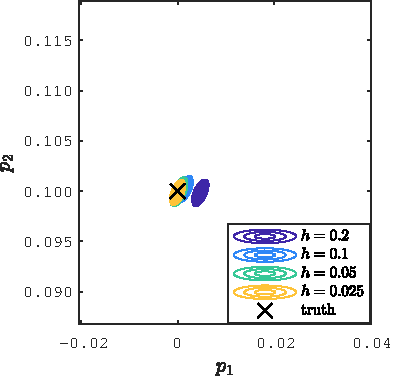
\includegraphics[width=0.4\linewidth]{BayesDet} & \includegraphics[width=0.4\linewidth]{BayesDet2} \\ 
			\end{tabular}
		\end{center}
	\end{figure}
	Posterior distributions given by {\color{NavyBlue} deterministic Störmer-Verlet method}.}

	\only<3>{
	\begin{figure}
		\begin{center}
			\begin{tabular}{c@{\hspace{0.3cm}}c}
				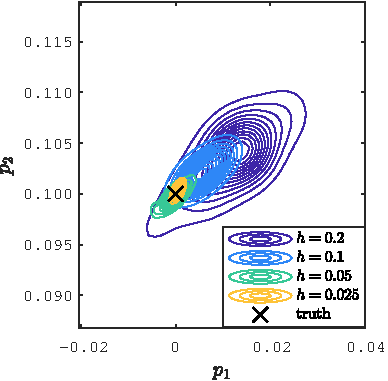
\includegraphics[width=0.4\linewidth]{BayesProb} & \includegraphics[width=0.4\linewidth]{BayesProb2} \\ 
			\end{tabular}
		\end{center}
	\end{figure}
	Posterior distributions given by {\color{ForestGreen} RTS-RK Störmer-Verlet method}.}
\end{frame}

\section{Research plan}

\begin{frame}
\frametitle{Research plan}
Future research will cover the following topics
\begin{itemize}
	\item Analysis of modelling errors in Bayesian inverse problems
	\item Probabilistic methods for PDEs, extension of the RTS-RK method?
	\item Adaptive time stepping probabilistic algorithms for ODEs
	\item Particle filter approach to sampling methods -- a bridge between sampling and filtering probabilistic methods
\end{itemize}
\end{frame}

\begin{frameT}
\frametitle{Research plan -- preliminary results}

\begin{figure}[t!]
	\begin{center}
		\begin{tabular}{cc}
			\includegraphics[width=0.25\textwidth]{solution1Def} & \includegraphics[width=0.25\textwidth]{solution2Def} \\
			\includegraphics[width=0.25\textwidth]{solution3Def} & \includegraphics[width=0.25\textwidth]{solution4Def} \\
		\end{tabular}
	\end{center}
\end{figure}

Probabilistic solutions of {\color{ForestGreen}$-\Delta u = sin(2\pi x)$} with random meshes.


\end{frameT}

\appendix
\begin{frame}[allowframebreaks, t]
	\frametitle{References}
	
	\setbeamertemplate{bibliography item}[text]
	\bibliographystyle{apalike}
	\bibliography{anmc}
\end{frame}

\end{document}
